\documentclass[prd,aps,nofootinbib,superscriptaddress,amsmath,amssymb]{revtex4}
\usepackage{amssymb,graphicx}
\usepackage{mathrsfs}
\usepackage[usenames,dvipsnames]{color}
\usepackage[bookmarks]{hyperref}
\usepackage{multirow, array}
\usepackage{float}

\newcommand{\Natural}{\mathbb{N}}
\newcommand{\Integer}{\mathbb{Z}}
\newcommand{\Real}{\mathbb{R}}
\newcommand{\Complex}{\mathbb{C}}
\newcommand{\re}{\mbox{Re}}
\newcommand{\im}{\mbox{Im}}

% Comments of the authors. Remove before submission.
\newcommand{\EJ}[1]{{\color{red}~\textsf{[(Erik) #1]}}}
\newcommand{\OS}[1]{{\color{blue}~\textsf{[(Olivier) #1]}}}

% Rows of the tables, generated by reproducir/scripts/reducido.py (python3 reducido.py tablas).
\newcommand{\TabReferencia}{%
$0.001$ & $0.10$ & $1.1\times 10^{-4}$ & $8.6\times 10^{-5}$ & $0.007$ & $0.007$ & -- & -- \\%
$0.01$ & $0.31$ & $2.4\times 10^{-3}$ & $2.4\times 10^{-3}$ & $0.061$ & $0.060$ & -- & -- \\%
$0.015$ & $0.37$ & $8.5\times 10^{-3}$ & $8.9\times 10^{-3}$ & $0.108$ & $0.104$ & -- & -- \\%
$0.02$ & $0.43$ & $1.2\times 10^{-2}$ & $7.5\times 10^{-3}$ & $0.160$ & $0.144$ & $0.103$ & $0.089$ \\%
$0.021$ & $0.44$ & $2.1\times 10^{-2}$ & $1.3\times 10^{-2}$ & $0.173$ & $0.154$ & $0.115$ & $0.100$ \\%
$0.022$ & $0.45$ & $3.0\times 10^{-2}$ & $2.0\times 10^{-2}$ & $0.182$ & $0.164$ & $0.129$ & $0.109$ \\%
$0.023$ & $0.46$ & $4.1\times 10^{-2}$ & $2.7\times 10^{-2}$ & $0.201$ & $0.172$ & $0.144$ & $0.122$ \\%
$0.024$ & $0.47$ & $5.8\times 10^{-2}$ & $3.5\times 10^{-2}$ & $0.218$ & $0.185$ & $0.154$ & $0.133$ \\%
$0.025$ & $0.48$ & $8.1\times 10^{-2}$ & $4.6\times 10^{-2}$ & $0.232$ & $0.199$ & $0.163$ & $0.143$ \\%
$0.03$ & $0.52$ & $0.22$ & $0.15$ & $0.276$ & $0.245$ & $0.232$ & $0.184$ \\%
$0.04$ & $0.60$ & $0.32$ & $0.23$ & $0.377$ & $0.337$ & $0.337$ & $0.256$ \\%
$0.05$ & $0.66$ & $0.19$ & $0.21$ & $0.450$ & $0.403$ & $0.376$ & $0.327$ \\%
$0.07$ & $0.76$ & $0.58$ & $0.46$ & $0.557$ & $0.493$ & $0.479$ & $0.415$ \\%
$0.1$ & $0.89$ & $0.85$ & $0.65$ & $0.290$ & $0.328$ & $0.516$ & $0.489$ \\%
\hline}

\newcommand{\TabFamilias}{%
Kepler & $0.01$ & $0.26$ & $1.1\times 10^{-3}$ & $9.7\times 10^{-4}$ & $0.036$ & $0.038$ & -- & -- \\%
 & $0.02$ & $0.37$ & $8.8\times 10^{-3}$ & $7.9\times 10^{-3}$ & $0.109$ & $0.104$ & -- & -- \\%
 & $0.04$ & $0.51$ & $0.23$ & $0.16$ & $0.284$ & $0.240$ & $0.234$ & $0.196$ \\%
 & $0.08$ & $0.69$ & $0.44$ & $0.23$ & $0.547$ & $0.435$ & $0.375$ & $0.360$ \\%
\hline%
$\sigma_J = 0.05$ & $0.005$ & $0.35$ & $8.3\times 10^{-3}$ & $8.4\times 10^{-3}$ & $0.092$ & $0.087$ & -- & -- \\%
 & $0.01$ & $0.49$ & $0.11$ & $8.9\times 10^{-2}$ & $0.232$ & $0.214$ & $0.186$ & $0.178$ \\%
 & $0.02$ & $0.69$ & $0.27$ & $0.26$ & $0.448$ & $0.410$ & $0.353$ & $0.334$ \\%
\hline%
$\sigma_J = 0.2$ & $0.02$ & $0.27$ & $7.1\times 10^{-4}$ & $4.9\times 10^{-4}$ & $0.037$ & $0.040$ & -- & -- \\%
 & $0.04$ & $0.38$ & $5.8\times 10^{-3}$ & $6.7\times 10^{-3}$ & $0.123$ & $0.109$ & -- & -- \\%
 & $0.08$ & $0.53$ & $0.33$ & $0.17$ & $0.345$ & $0.251$ & $0.309$ & $0.200$ \\%
\hline%
$\sigma_Q = 0.2$ & $0.01$ & $0.30$ & $1.5\times 10^{-3}$ & $1.4\times 10^{-3}$ & $0.048$ & $0.048$ & -- & -- \\%
 & $0.02$ & $0.42$ & $7.4\times 10^{-3}$ & $8.3\times 10^{-3}$ & $0.134$ & $0.123$ & $0.059$ & $0.050$ \\%
 & $0.04$ & $0.58$ & $0.14$ & $9.4\times 10^{-2}$ & $0.332$ & $0.282$ & $0.199$ & $0.169$ \\%
 & $0.08$ & $0.78$ & $0.24$ & $0.12$ & $0.536$ & $0.486$ & $0.289$ & $0.250$ \\%
\hline%
$\sigma_Q = 0.4$ & $0.01$ & $0.27$ & $5.1\times 10^{-4}$ & $4.2\times 10^{-4}$ & $0.027$ & $0.026$ & -- & -- \\%
 & $0.02$ & $0.38$ & $4.8\times 10^{-3}$ & $4.2\times 10^{-3}$ & $0.075$ & $0.068$ & -- & -- \\%
 & $0.04$ & $0.52$ & $1.4\times 10^{-2}$ & $8.4\times 10^{-3}$ & $0.184$ & $0.157$ & $0.082$ & $0.071$ \\%
 & $0.08$ & $0.69$ & $0.10$ & $4.4\times 10^{-2}$ & $0.336$ & $0.282$ & $0.122$ & $0.114$ \\%
\hline}

\newcommand{\TabL}{%
$0.03$ & $0$ & $0.00$ & $1$ & $0.15$ & $5.74$ & $0.248$ & $0.195$ \\%
$0.03$ & $0.005$ & $0.18$ & $4$ & $0.12$ & $4.61$ & $0.244$ & $0.181$ \\%
$0.03$ & $0.01$ & $0.35$ & $6$ & $3.6\times 10^{-2}$ & $3.66$ & $0.243$ & $0.147$ \\%
$0.03$ & $0.02$ & $0.71$ & $10$ & $1.5\times 10^{-3}$ & $2.05$ & $0.211$ & $0.078$ \\%
$0.03$ & $0.04$ & $1.41$ & $20$ & $4.1\times 10^{-4}$ & $0.59$ & $0.140$ & $0.037$ \\%
$0.01$ & $0$ & $0.00$ & $1$ & $2.5\times 10^{-3}$ & $0.06$ & $0.057$ & $0.042$ \\%
$0.01$ & $0.02$ & $0.71$ & $10$ & $1.4\times 10^{-4}$ & $0.04$ & $0.045$ & $0.031$ \\%
\hline}

\newcommand{\TabLargas}{%
$0.02$ & $200\times 50$ & $223$ & $0.008$ & $0.012$ & $0.017$ & $0.079$ & $0.075$ & $0.081$ \\%
$0.02$ & $300\times 75$ & $502$ & $0.007$ & $0.010$ & $0.014$ & $0.037$ & $0.051$ & $0.057$ \\%
$0.02$ & $400\times 100$ & $892$ & $0.007$ & $0.011$ & $0.015$ & $0.036$ & $0.037$ & $0.045$ \\%
$0.022$ & $400\times 100$ & $892$ & $0.020$ & $0.027$ & $0.062$ & $0.049$ & $0.047$ & $0.050$ \\%
$0.025$ & $200\times 50$ & $223$ & $0.051$ & $0.104$ & $0.106$ & $0.086$ & $0.111$ & $0.088$ \\%
$0.025$ & $300\times 75$ & $502$ & $0.045$ & $0.099$ & $0.076$ & $0.086$ & $0.101$ & $0.079$ \\%
$0.025$ & $400\times 100$ & $892$ & $0.046$ & $0.099$ & $0.068$ & $0.079$ & $0.056$ & $0.059$ \\%
$0.03$ & $400\times 100$ & $892$ & $0.155$ & $0.118$ & $0.091$ & $0.100$ & $0.096$ & $0.070$ \\%
\hline}



%%%%%%%%%%%%%%%%%%%%%%%%%%%%%%%
\begin{document}
%%%%%%%%%%%%%%%%%%%%%%%%%%%%%%%


\title{A reduced model for the phase space mixing of a self-gravitating gas cloud near the circular orbit}

\author{Erik Jim\'enez-V\'azquez}
\affiliation{\EJ{Affiliation to be completed.}}

\author{Olivier Sarbach}
\affiliation{Instituto de F\'isica y Matem\'aticas,
Universidad Michoacana de San Nicol\'as de Hidalgo,
Edificio C-3, Ciudad Universitaria, 58040 Morelia, Michoac\'an, M\'exico}


\begin{abstract}
These notes contain the derivation of a reduced model for a spherically symmetric, collisionless gas cloud which is trapped in an external central potential, whose particles move on nearly circular orbits and whose self-gravity is taken into account. To leading order in the eccentricity of the orbits two gas shells interact like two parallel sheets, and the average over the radial oscillation yields a Hamiltonian system for the complex amplitudes of these oscillations, in which the interaction energy of two shells with the same angular momentum is proportional to the distance between their amplitudes. For a cloud of a given shape the model contains a single parameter, whose square root is proportional to the parameter $\mu$ of the main notes. The model is compared, without adjusting any parameter, with $48$ particle-in-cell simulations of the cloud in which all the particles have the same angular momentum. It reproduces the frequencies of the relaxed states, the mass which accumulates near the circular orbit, the formation of a dense core and the decay and the revival of its oscillation. When the angular momenta of the gas particles are distributed, two shells only interact when they cross each other, which softens the interaction. In this case the model predicts that the core and its oscillation disappear when the relative width of the distribution of the angular momenta exceeds about one percent; this prediction has not been compared with simulations yet.
\end{abstract}

\date{\today}

\maketitle


%%%%%%%%%%%%%%%%%%%%%%%%%%%%%%%%%%%%%%%%%%%%%
\section{Introduction}
\label{Sec:Intro}
%%%%%%%%%%%%%%%%%%%%%%%%%%%%%%%%%%%%%%%%%%%%%

In the main notes\EJ{``The main notes'' are the article in docs/articulo, whose notation is used here. The cross references have to be replaced when both texts are merged.} we study numerically, by means of a particle-in-cell (PIC) code, the relaxation of a spherically symmetric gas cloud which is trapped in an external central potential and which is initially concentrated about one orbital phase, taking into account the self-gravity of the gas. In the reduced model in which all the gas particles have the same magnitude $L_0$ of the angular momentum, the outcome is controlled by a parameter $\mu$ which compares the amplitude of the potential generated by the cloud with the spread of its orbital frequencies. For small $\mu$ the cloud mixes, although the state which is reached differs from the average of the initial distribution function (DF) over the angle variable; for larger $\mu$ a dense core is left at the circular orbit, and its radial oscillation becomes more persistent as $\mu$ grows. In the main notes the parameter $\mu$ is introduced through a heuristic argument, and no explanation is given for the formation of the core, for the frequency of its oscillation or for the dependence of the results on the shape of the cloud.

The purpose of these notes is to derive a reduced model which provides such an explanation. It rests on two observations. First, the orbits of the cloud have a small eccentricity, such that all the gas shells stay close to the radius of the circular orbit, and to leading order two such shells attract each other like two parallel sheets, with a force which does not depend on their distance. Second, the self-gravity of the cloud and the differences between the orbital frequencies act on a time scale which is long compared with the period of the radial oscillation, such that the interaction can be averaged over this oscillation. The result is a Hamiltonian system for the complex amplitudes of the radial oscillations of the shells. For a cloud of a given shape it contains a single parameter, it can be solved numerically at a much lower cost than the full problem, and several quantities which are measured in the PIC simulations can be computed from it in closed form.

The self-gravitating sheet model has been used to study the collisionless relaxation of one-dimensional systems; in particular, it leads to quasi-stationary states which consist of a dense core surrounded by a dilute halo~\cite{mJtW11,yLrPfRtTfB14}. The same interaction describes the motion of the stars perpendicular to the plane of a galactic disk, and in this context it has been found that the self-gravity of the disk delays the phase mixing of a perturbation and may leave a spiral structure in phase space which is almost undamped~\cite{kDlW19,lW23,tAtA26}. The model derived in these notes describes the same interaction in the presence of an external potential which dominates the dynamics, and after the average over the fast oscillation it has the structure of the equations for a two-dimensional incompressible fluid, in which the mass density in the plane of the complex amplitudes plays the role of the vorticity. In that context, the damping of a mode of a vortex through its resonance with the co-rotating fluid and the migration of a vortex in a background shear flow have been analyzed in Refs.~\cite{dSdDaCcDiLtO00,dSdD01}, and the weakly damped oscillation of the core which we find below has an analogue in spherical stellar systems~\cite{mW94}.

These notes are organized as follows. In section~\ref{Sec:Shells} we formulate the dynamics of the gas shells and expand their interaction near the circular orbit. In section~\ref{Sec:FixedL} we derive the reduced model for shells with the same angular momentum, identify its parameter and its relation with $\mu$, and obtain the frequencies of the mixed states and of the oscillation of a compact core. In section~\ref{Sec:DistL} the model is extended to a gas whose angular momenta are distributed. The numerical solution of the model is described in section~\ref{Sec:Numerics}, and in section~\ref{Sec:Comparison} it is compared with the PIC simulations. Conclusions are drawn in section~\ref{Sec:Conclusions}. We use the dimensionless variables of the main notes, in which $G = M = b = 1$ for the isochrone potential and $G = M = 1$ for the Kepler potential, although we keep Newton's constant $G$ in the formulas.


%%%%%%%%%%%%%%%%%%%%%%%%%%%%%%%%%%%%%%%%%%%%%
\section{Gas shells near the circular orbit}
\label{Sec:Shells}
%%%%%%%%%%%%%%%%%%%%%%%%%%%%%%%%%%%%%%%%%%%%%

In this section we write the equations of motion of the gas shells in Hamiltonian form and expand the interaction between two shells which are close to the same radius.

As in the PIC method, we represent the gas by $N$ spherical shells with radii $r_j(t)$, radial momenta per unit mass $p_j(t)$, angular momenta per unit mass $L_j$ and masses $m_j$, $j = 1,2,\ldots,N$. Their equations of motion are
\begin{equation}
\frac{dr_j}{dt} = p_j,\qquad
\frac{dp_j}{dt} = \frac{L_j^2}{r_j^3} - \frac{\partial\Phi_{ext}}{\partial r}(r_j) - \frac{G m(t,r_j)}{r_j^2},
\label{Eq:EOM}
\end{equation}
where $m(t,r)$ denotes the mass of the gas inside the sphere of radius $r$ at time $t$. These are Hamilton's equations for the function
\begin{equation}
H = \sum\limits_{j=1}^N m_j\left[ \frac{p_j^2}{2} + \frac{L_j^2}{2r_j^2} + \Phi_{ext}(r_j) \right]
 - G\sum\limits_{i<j} \frac{m_i m_j}{\max\{ r_i,r_j \}},
\label{Eq:HShells}
\end{equation}
with respect to the canonical pairs $(r_j,m_j p_j)$: the derivative of the last term with respect to $r_i$ yields the mass of the shells which lie inside the shell $i$, divided by $r_i^2$.\footnote{A shell is also attracted by half of its own mass, which corresponds to the additional term $-G\sum_j m_j^2/(2r_j)$ in Eq.~(\ref{Eq:HShells}). Its contribution vanishes in the limit $N\to \infty$ with fixed total mass, and it plays no role in what follows.} In the limit $N\to \infty$, $H$ is the energy of the gas given in the main notes.

In the absence of self-gravity each shell moves in the effective potential $V_L(r) = \Phi_{ext}(r) + L^2/(2r^2)$, and its motion is described by the action-angle variables $(Q,J)$ of the external potential, in terms of which the energy per unit mass is $E(J,L)$ and the frequency of the radial motion is $\Omega(J,L) = \partial E/\partial J$. We denote by $R(L)$ the radius of the circular orbit with angular momentum $L$, which is the minimum of $V_L$, and by
\begin{equation}
\kappa(L) := \Omega(0,L) = \sqrt{V_L''(R(L))}
\label{Eq:kappa}
\end{equation}
the frequency of the small radial oscillations about it. For nearly circular orbits,
\begin{equation}
r = R(L) - \left( \frac{2J}{\kappa(L)} \right)^{1/2}\cos Q + \mathcal{O}(J),\qquad
p_r = \left( 2\kappa(L) J \right)^{1/2}\sin Q + \mathcal{O}(J),
\label{Eq:Epicycle}
\end{equation}
where the sign of the first term is due to the convention $Q = 0$ at the pericenter. For the isochrone and the Kepler potentials one has $E(J,L) = -[J + c(L)]^{-2}/2$ and $\Omega(J,L) = [J + c(L)]^{-3}$ with $c(L) = (L + \sqrt{L^2 + 4})/2$ and $c(L) = L$, respectively, and thus
\begin{equation}
\kappa(L) = \frac{1}{c(L)^3},\qquad
R(L) = \sqrt{c(L)^4 - 1}\quad\hbox{(isochrone)},\qquad
R(L) = L^2\quad\hbox{(Kepler)}.
\label{Eq:RkappaIsochrone}
\end{equation}

Let $L_0$ be a reference value of the angular momentum, $R_0 := R(L_0)$ and $\kappa_0 := \kappa(L_0)$, and suppose that all the shells remain close to the radius $R_0$, that is,
\begin{equation}
r_j = R_0 + \xi_j,\qquad |\xi_j|\ll R_0.
\label{Eq:xiDef}
\end{equation}
Using $\max\{ a,b \} = (a + b + |a - b|)/2$, the interaction energy of two shells is
\begin{equation}
-\frac{G m_i m_j}{\max\{ r_i,r_j \}} = -\frac{G m_i m_j}{R_0}
 + \frac{G m_i m_j}{2R_0^2}\left( \xi_i + \xi_j \right)
 + \frac{G m_i m_j}{2R_0^2}\left| \xi_i - \xi_j \right|
 + \mathcal{O}\left( \frac{\xi^2}{R_0^3} \right).
\label{Eq:PairExpansion}
\end{equation}
The first term on the right-hand side is a constant. The sum of the second one over all the pairs is $G\sum_j m_j(M_{gas} - m_j)\xi_j/(2R_0^2)$: each shell is subject to a constant force, as if half of the mass of the remaining gas was located at the center. This force displaces the circular orbits inwards and, as shown in section~\ref{SubSec:Mixed}, it shifts the frequencies of all the shells by the same amount; hence it does not affect the motion of the shells relative to each other. The third term is the interaction energy of two parallel sheets with the surface densities $m_i/(4\pi R_0^2)$ and $m_j/(4\pi R_0^2)$ and the area $4\pi R_0^2$. It gives rise to a force between the two shells which is independent of their distance and which changes its sign when they cross. This term contains the collective dynamics of the cloud, and the reduced model is obtained from it.


%%%%%%%%%%%%%%%%%%%%%%%%%%%%%%%%%%%%%%%%%%%%%
\section{The reduced model for shells with the same angular momentum}
\label{Sec:FixedL}
%%%%%%%%%%%%%%%%%%%%%%%%%%%%%%%%%%%%%%%%%%%%%

In this section we assume that $L_j = L_0$ for all the shells and write $E(J)$ and $\Omega(J)$ for $E(J,L_0)$ and $\Omega(J,L_0)$. We average the interaction over the radial oscillation, identify the parameter of the resulting model, and derive the frequencies of its stationary states and of the oscillation of a compact core.


\subsection{Average over the radial oscillation}
\label{SubSec:Average}

We describe the state of the shell $j$ by the complex amplitude of its radial oscillation in a frame which rotates with the frequency $\kappa_0$ of the circular orbit,
\begin{equation}
\zeta_j := \sqrt{2J_j}\, e^{i(Q_j - \kappa_0 t)},
\label{Eq:zetaDef}
\end{equation}
where $(Q_j,J_j)$ are the action-angle variables of the external potential. In the absence of self-gravity $J_j$ is constant and $Q_j$ advances with the frequency $\Omega(J_j)$, such that $\dot{\zeta}_j = i[\Omega(J_j) - \kappa_0]\zeta_j$. According to Eqs.~(\ref{Eq:Epicycle},\ref{Eq:xiDef}),
\begin{equation}
\xi_i - \xi_j = -\frac{1}{\sqrt{\kappa_0}}\,\re\left[ \left( \zeta_i - \zeta_j \right) e^{i\kappa_0 t} \right] + \mathcal{O}(J).
\label{Eq:xiDiff}
\end{equation}
Suppose that the amplitudes $\zeta_j$ change little during one period $2\pi/\kappa_0$ of the radial oscillation. This requires that the frequencies of the orbits of the cloud differ little from $\kappa_0$ and that the self-gravity of the gas is weak, in the sense made precise below. In this case the interaction can be replaced by its average over one period at fixed amplitudes. Since the average of $|\cos\theta|$ over $\theta$ is $2/\pi$, Eq.~(\ref{Eq:xiDiff}) yields
\begin{equation}
\left\langle \left| \xi_i - \xi_j \right| \right\rangle = \frac{2}{\pi\sqrt{\kappa_0}}\left| \zeta_i - \zeta_j \right|,
\label{Eq:AverageFixedL}
\end{equation}
and the Hamiltonian~(\ref{Eq:HShells}) is replaced with the reduced Hamiltonian
\begin{equation}
\overline{H} = \sum\limits_{j=1}^N m_j\left[ E(J_j) - \kappa_0 J_j \right] + g\sum\limits_{i<j} m_i m_j\left| \zeta_i - \zeta_j \right|,\qquad
g := \frac{G}{\pi R_0^2\sqrt{\kappa_0}},
\label{Eq:Hred}
\end{equation}
where $J_j = |\zeta_j|^2/2$, the term $-\kappa_0 J_j$ is due to the rotating frame, and the constant and the uniform force of Eq.~(\ref{Eq:PairExpansion}) have been omitted. The canonical pairs are $(\vartheta_j,m_j J_j)$ with $\vartheta_j := Q_j - \kappa_0 t$ the argument of $\zeta_j$, which is equivalent to $m_j\dot{\zeta}_j = 2i\,\partial\overline{H}/\partial\zeta_j^*$. This yields the equations of motion
\begin{equation}
\frac{d\zeta_i}{dt} = i\left[ \Omega(J_i) - \kappa_0 \right]\zeta_i
 + i g\sum\limits_{j\neq i} m_j\frac{\zeta_i - \zeta_j}{|\zeta_i - \zeta_j|},\qquad i = 1,2,\ldots,N,
\label{Eq:Reduced}
\end{equation}
which constitute the reduced model. Besides $\overline{H}$, it conserves the quantity
\begin{equation}
P := \sum\limits_{j=1}^N m_j J_j,
\label{Eq:PDef}
\end{equation}
since $\overline{H}$ is invariant with respect to a common rotation of all the amplitudes.

In the limit $N\to \infty$ the gas is described by the mass density $n(t,\zeta)$ in the plane of the amplitudes, such that $n\, d^2\zeta$ with $d^2\zeta = d\vartheta\, dJ$ is the mass in the corresponding area element; in terms of the DF of the reduced model of the main notes, $n = 8\pi^2 L_0\mathcal{F}_0$. Equation~(\ref{Eq:Reduced}) is then replaced with
\begin{equation}
\frac{\partial n}{\partial t} + \frac{\partial\mathcal{H}}{\partial J}\frac{\partial n}{\partial\vartheta} - \frac{\partial\mathcal{H}}{\partial\vartheta}\frac{\partial n}{\partial J} = 0,\qquad
\mathcal{H}(t,\zeta) := E(J) - \kappa_0 J + g\int \left| \zeta - \zeta' \right| n(t,\zeta')\, d^2\zeta'.
\label{Eq:ReducedVlasov}
\end{equation}
For $g = 0$ this is the Vlasov equation in action-angle variables of the main notes, written in the rotating frame.

Equation~(\ref{Eq:ReducedVlasov}) states that the density $n$ is transported by an area-preserving flow in the $\zeta$-plane whose stream function $\mathcal{H}$ consists of a prescribed part and of a part which is generated by $n$ itself. This is the structure of the equation for the vorticity of a two-dimensional incompressible fluid, with the kernel $|\zeta - \zeta'|$ in place of the logarithmic one. The prescribed part describes a differential rotation about the origin with the angular velocity $\Omega(J) - \kappa_0$, which vanishes at $\zeta = 0$ and which is negative elsewhere, since $\Omega$ decreases with $J$. In contrast to this, a concentration of gas induces a rotation about itself in the positive sense, since the kernel grows with the distance: the self-gravity raises the frequencies of the neighboring orbits. Two consequences can be read off directly. First, a concentration of gas at $\zeta = 0$, that is, at the circular orbit, is not sheared by the differential rotation, which explains why the core found in the main notes is located there. Second, a compact cloud which is placed at a distance from the origin rotates about its own center, and this rotation transports the part of the cloud which leads in the angle variable towards the origin.

The assumptions made in the derivation are the following: (i) the eccentricity of the orbits is small, such that Eqs.~(\ref{Eq:Epicycle},\ref{Eq:PairExpansion}) can be truncated; the relevant parameter is the ratio between the amplitude of the radial oscillation and $R_0$; (ii) $|\Omega(J) - \kappa_0|\ll\kappa_0$ over the support of the cloud; (iii) the rotation which is induced by the gas, of the order of $g M_{gas}/|\zeta|$, is small compared with $\kappa_0$. For the cloud of the main notes with $\sigma_J = 0.1$ and $L_0 = 2$ in the isochrone potential one has $R_0 = 5.742$, $\kappa_0 = 0.07107$ and $g = 0.03621$; the ratio in (i) is $(2\sigma_J/\kappa_0)^{1/2}/R_0 = 0.29$, the one in (ii) is $0.12$ at $J = \sigma_J$ and $0.28$ at the lower end of the frequency band, and the one in (iii) is $0.02$ for $M_{gas}/M = 0.02$. Hence, the first assumption is the most restrictive one. In Eq.~(\ref{Eq:Reduced}) we keep the exact frequency $\Omega(J)$ of the external potential, such that the model reproduces the mixing of the cloud without self-gravity exactly.


\subsection{Scaling and the parameter $\mu$}
\label{SubSec:Scaling}

Let $\sigma_J$ be the scale of the action variables of the cloud. To leading order in $\sigma_J$, $\Omega(J) - \kappa_0 = \Omega_0' J$ with $\Omega_0' := \partial\Omega/\partial J(0,L_0) < 0$. Introducing the rescaled quantities $\tilde{\zeta}_j := \zeta_j/\sqrt{\sigma_J}$, $\tilde{J}_j := J_j/\sigma_J$, $\tilde{t} := |\Omega_0'|\sigma_J t$ and $\tilde{m}_j := m_j/M_{gas}$, Eq.~(\ref{Eq:Reduced}) assumes the form
\begin{equation}
\frac{d\tilde{\zeta}_i}{d\tilde{t}} = -i\tilde{J}_i\tilde{\zeta}_i
 + i\,\Gamma\sum\limits_{j\neq i} \tilde{m}_j\frac{\tilde{\zeta}_i - \tilde{\zeta}_j}{|\tilde{\zeta}_i - \tilde{\zeta}_j|},\qquad
\Gamma := \frac{g M_{gas}}{|\Omega_0'|\,\sigma_J^{3/2}} = \frac{G M_{gas}}{\pi R_0^2\,\kappa_0^{1/2}\,|\Omega_0'|\,\sigma_J^{3/2}}.
\label{Eq:Gamma}
\end{equation}
For the cloud of the main notes, whose initial density is proportional to $\exp[-\sin^2(Q/2)/\sigma_Q^2]\tilde{J}^2\exp(-\tilde{J}^2)$, the initial datum in the rescaled variables only depends on $\sigma_Q$. Therefore, to leading order the evolution of the cloud is determined by the parameter $\Gamma$ and by its width in the angle variable; the mass of the gas, its width in the action variable, the angular momentum and the external potential only enter through $\Gamma$ and through the unit $1/(|\Omega_0'|\sigma_J)$ of time, which is proportional to the mixing time $\tau_1$ of the main notes.

The parameter $\Gamma$ is related to $\mu$ as follows. A compact cloud with action variable $J$ oscillates between the radii $R_0\mp a$ with $a = (2J/\kappa_0)^{1/2}$. At a fixed radius $r$ in this range the potential which it generates varies between $-GM_{gas}/r$ and $-GM_{gas}/(R_0 + a)$, and half of the largest variation is $A = GM_{gas}a/R_0^2$ to leading order. With $J = \sigma_J$ this gives
\begin{equation}
A = \frac{GM_{gas}}{R_0^2}\left( \frac{2\sigma_J}{\kappa_0} \right)^{1/2} = \pi g M_{gas}\sqrt{2\sigma_J},
\label{Eq:AReduced}
\end{equation}
which is $0.0509\, M_{gas}/M$ for the reference cloud, in agreement with the value $0.0496\, M_{gas}/M$ measured in the PIC simulations. Since $\mu^2 = A/(|\Omega'|\Delta J^2)$ with $\Delta J = 2.70\,\sigma_J$ the width of the support of the cloud, it follows that
\begin{equation}
\mu^2 = \frac{\sqrt{2}\,\pi}{2.70^2}\,\Gamma = 0.61\,\Gamma.
\label{Eq:muGamma}
\end{equation}
Therefore, $\mu$ is, up to a numerical factor, the square root of the only parameter of the reduced model. For the reference cloud in the isochrone potential $\Omega_0' = -0.08831$ and $\Gamma = 12.97\, M_{gas}/M$, and in the Kepler potential with $L_0 = 2$ one has $R_0 = 4$, $\kappa_0 = 1/8$, $\Omega_0' = -3/16$, $g = 0.05627$ and $\Gamma = 9.49\, M_{gas}/M$. The values of $\mu$ which follow from Eq.~(\ref{Eq:muGamma}) are about $8$ percent smaller than those of the main notes, where $|\Omega'|$ is the mean slope $\Delta\Omega/\Delta J$ of the frequency over the band instead of its value at the circular orbit.

The reduced model also makes the heuristic argument of the main notes more precise. For a cloud which is compact in the angle variable and whose center has the action variable $J_c$, a gas particle with the same action variable and with the angle $\vartheta$ relative to the center has the interaction energy $g M_{gas}|\zeta - \zeta_c| = 2gM_{gas}\sqrt{2J_c}\,|\sin(\vartheta/2)|$ per unit mass. With $J_c = \sigma_J$ and Eq.~(\ref{Eq:AReduced}), the depth of this potential well is $2A/\pi$, instead of the depth $2A$ of the pendulum considered in the main notes, and the half-width of its separatrix in the action variable is $(2/\sqrt{\pi})(A/|\Omega'|)^{1/2} = (2/\sqrt{\pi})\,\mu\,\Delta J$. It covers the support of the cloud, $\Delta J/2$ on each side of its center, when
\begin{equation}
\mu\geq \frac{\sqrt{\pi}}{4}\approx 0.44.
\label{Eq:muEstimate}
\end{equation}
This value lies in the range $0.43\leq\mu\leq 0.48$ in which the PIC simulations of the clouds that are compact in the angle variable change from a relaxed state to a persistent oscillation of the core. However, the estimate depends on the convention for the width of the support, it treats the potential of the cloud as rigid, and it does not explain why a cloud which is wide in the angle variable requires a larger value of $\mu$; these features are only obtained from the solution of Eq.~(\ref{Eq:Reduced}), see section~\ref{Sec:Comparison}.


\subsection{Mixed states and their frequencies}
\label{SubSec:Mixed}

Any density which only depends on the action variable, $n = \hat{n}(J)$, is a stationary solution of Eq.~(\ref{Eq:ReducedVlasov}), since in this case $\mathcal{H}$ is independent of $\vartheta$. These are the mixed states of the reduced model. The average of $|\zeta - \zeta'|$ over the argument of $\zeta'$ at fixed moduli $\rho := |\zeta|$ and $\rho' := |\zeta'|$ is $(2/\pi)(\rho + \rho')\mathbf{E}(k)$ with $k^2 := 4\rho\rho'/(\rho + \rho')^2$, where $\mathbf{E}(k) := \int_0^{\pi/2}(1 - k^2\sin^2\theta)^{1/2} d\theta$ denotes the complete elliptic integral of the second kind. Hence,
\begin{equation}
\mathcal{H} = E(J) - \kappa_0 J + g\,\psi(\rho),\qquad
\psi(\rho) := \frac{2}{\pi}\int\limits_0^\infty (\rho + \rho')\,\mathbf{E}\left( \frac{2\sqrt{\rho\rho'}}{\rho + \rho'} \right) \hat{n}\, 2\pi\rho'\, d\rho',
\label{Eq:psiMixed}
\end{equation}
and since $J = \rho^2/2$ the frequency of the gas particles with action variable $J$ is
\begin{equation}
\Omega_{tot}(J) = \Omega(J) + \frac{g}{\rho}\frac{d\psi}{d\rho}(\rho),\qquad \rho = \sqrt{2J}.
\label{Eq:OmegaTot}
\end{equation}
The second term is positive: the gas raises the frequencies. A ring of mass $m'$ with radius $\rho'$ contributes $g m'/(2\rho')$ to the frequency of the orbits inside it ($\rho\ll\rho'$) and $g m'/\rho$ to the one of the orbits far outside it ($\rho\gg\rho'$).

Equation~(\ref{Eq:OmegaTot}) only contains the contribution of the last term in Eq.~(\ref{Eq:PairExpansion}). At first order in the mass of the gas there is a further contribution, which is due to the uniform force and to the terms of the next order in $\xi/R_0$. For the nearly circular orbits it is obtained from the frequency of the small oscillations about the minimum $r_*$ of the time-averaged effective potential, $\kappa_{tot}^2 = V_{L_0}''(r_*) + G[\overline{m}'(r_*)/r_*^2 - 2\overline{m}(r_*)/r_*^3]$, where $\overline{m}(r)$ is the time average of the mass of the gas inside the radius $r$ and $r_* - R_0 = -G\overline{m}(R_0)/(R_0^2\kappa_0^2)$ to first order. The term with $\overline{m}'$ is the one contained in Eq.~(\ref{Eq:OmegaTot}), and the remaining ones give the shift
\begin{equation}
\delta\Omega_u = -\frac{G\,\overline{m}(R_0)}{2\kappa_0}\left[ \frac{V_{L_0}'''(R_0)}{R_0^2\kappa_0^2} + \frac{2}{R_0^3} \right],
\label{Eq:UniformShift}
\end{equation}
which is $0.1454\,\overline{m}(R_0)$ for the isochrone potential with $L_0 = 2$ and $2\overline{m}(R_0)/L_0^3$ for the Kepler potential. In section~\ref{Sec:Comparison} we show that in the PIC simulations this shift is the same for all the gas particles within $5$ percent. A uniform shift of the frequencies amounts to a change of $\kappa_0$ in Eq.~(\ref{Eq:zetaDef}) and does not affect the reduced dynamics.


\subsection{Oscillation of a compact core}
\label{SubSec:Core}

Suppose that the gas consists of a compact core of mass $m_c$ close to $\zeta = 0$ and of a halo which is mixed, and let $\zeta_c := \sum_j m_j\zeta_j/m_c$ be the center of the core, where the sum extends over its particles. Since the interaction term in Eq.~(\ref{Eq:Reduced}) is antisymmetric in the two particles, the forces between the particles of the core cancel in the motion of its center. The remaining terms are the differential rotation and the interaction with the halo, which are described by a stream function $\mathcal{H}_h(J)$ of the form~(\ref{Eq:psiMixed}) with the density of the halo. If the extension of the core and its displacement are small compared with the scale on which $d\mathcal{H}_h/dJ$ varies, Eq.~(\ref{Eq:Reduced}) yields $\dot{\zeta}_c = i[\Omega_h(0) - \kappa_0]\zeta_c$, where $\Omega_h(J)$ is given by Eq.~(\ref{Eq:OmegaTot}) with the density of the halo. Therefore, the core oscillates like a rigid body about the circular orbit with the frequency
\begin{equation}
\omega_c = \Omega_h(0) + \delta\Omega_u,
\label{Eq:omegac}
\end{equation}
which is the frequency of the nearly circular orbits in the field of the halo alone. It depends neither on the mass of the core nor on its internal structure. This is analogous to the motion of the center of mass of a system of interacting particles in a harmonic trap.

The frequencies of the individual gas particles differ from $\omega_c$. A particle inside the core is also subject to the field of the core, which raises its frequency above $\omega_c$. A particle of the halo at the distance $\rho = \sqrt{2J}$ from the core, with $\rho$ large compared with the extension of the core, has the frequency $\Omega_h(J) + g m_c/\rho$, which exceeds $\omega_c$ close to the core and falls below it further out, since $\Omega_h$ decreases with $J$. With $\Omega_h(J) - \Omega_h(0) = \Omega_0' J$, both frequencies coincide at
\begin{equation}
J_{res} = \left( \frac{g m_c}{\sqrt{2}\,|\Omega_0'|} \right)^{2/3}.
\label{Eq:Jres}
\end{equation}
The particles with $J\approx J_{res}$ co-rotate with the displacement of the core and can exchange energy with its oscillation. For $|\zeta|\gg|\zeta_c|$ the displacement of the core changes the stream function of a particle of the halo by $-g m_c|\zeta_c|\cos(\vartheta - \vartheta_c)$, with $\vartheta_c$ the argument of $\zeta_c$, whose amplitude does not depend on $J$. In the frame which rotates with the core this is the Hamiltonian of a pendulum near $J_{res}$, as in the theory of the damping of a plasma wave by the particles which are in resonance with it~\cite{tO65}. Since $d(\Omega_h + g m_c/\rho)/dJ = 3\Omega_0'/2$ at $J = J_{res}$, the frequency of the small oscillations of the trapped particles is
\begin{equation}
\omega_b = \left( \frac{3}{2}\, g m_c |\zeta_c|\, |\Omega_0'| \right)^{1/2},
\label{Eq:omegab}
\end{equation}
and the half-width of the resonance in the action variable is $2\omega_b/(3|\Omega_0'|/2)$. According to this picture, the oscillation of the core can only be damped by the gas particles close to $J_{res}$, at a rate which is determined by the slope of their distribution, and the damping is modified after a time of the order of $2\pi/\omega_b$, when these particles have been trapped. We have not derived the damping rate; the comparison of section~\ref{Sec:Comparison} only refers to the frequency~(\ref{Eq:omegac}), to the location~(\ref{Eq:Jres}) of the resonance and to the order of magnitude of $2\pi/\omega_b$.


%%%%%%%%%%%%%%%%%%%%%%%%%%%%%%%%%%%%%%%%%%%%%
\section{Distributed angular momenta}
\label{Sec:DistL}
%%%%%%%%%%%%%%%%%%%%%%%%%%%%%%%%%%%%%%%%%%%%%

In this section we extend the reduced model to a gas whose particles have different angular momenta $L_j$, distributed about $L_0$ with a width $\sigma_L\ll L_0$.

Two properties of the shells now depend on $j$: the frequency $\Omega(J_j,L_j)$ of the radial motion and the radius $R(L_j)$ of the circular orbit about which the shell oscillates. We define the amplitudes $\zeta_j$ by Eq.~(\ref{Eq:zetaDef}) with the same frequency $\kappa_0 = \kappa(L_0)$ for all the shells, such that the differences $\kappa(L_j) - \kappa_0$ appear as a slow rotation of $\zeta_j$. Replacing $\kappa(L_j)$ with $\kappa_0$ in the amplitude of Eq.~(\ref{Eq:Epicycle}), which introduces a relative error of the order of $\sigma_L/L_0$, Eq.~(\ref{Eq:xiDiff}) is replaced with
\begin{equation}
\xi_i - \xi_j = D_{ij} - \frac{1}{\sqrt{\kappa_0}}\,\re\left[ \left( \zeta_i - \zeta_j \right) e^{i\kappa_0 t} \right],\qquad
D_{ij} := R(L_i) - R(L_j).
\label{Eq:xiDiffL}
\end{equation}
The average of $|D - \rho\cos\theta|$ over $\theta$ is equal to $|D|$ when $|D|\geq\rho$, since in this case the expression inside the modulus does not change its sign, and to $(2/\pi)[(\rho^2 - D^2)^{1/2} + D\arcsin(D/\rho)]$ when $|D| < \rho$. Therefore,
\begin{equation}
\left\langle \left| \xi_i - \xi_j \right| \right\rangle = \frac{2}{\pi\sqrt{\kappa_0}}\,\mathcal{G}\left( |\zeta_i - \zeta_j|,d_{ij} \right),\qquad
d_{ij} := \sqrt{\kappa_0}\left[ R(L_i) - R(L_j) \right],
\label{Eq:AverageL}
\end{equation}
with the function
\begin{equation}
\mathcal{G}(\rho,d) := \left\{ \begin{array}{ll}
\sqrt{\rho^2 - d^2} + d\arcsin\left( \displaystyle\frac{d}{\rho} \right), & |d| < \rho,\\
\displaystyle\frac{\pi}{2}|d|, & |d|\geq\rho,
\end{array} \right.
\label{Eq:Kernel}
\end{equation}
which reduces to $\rho$ for $d = 0$ and which is continuously differentiable, with $\partial\mathcal{G}/\partial\rho = (1 - d^2/\rho^2)^{1/2}$ for $|d| < \rho$. The reduced Hamiltonian is
\begin{equation}
\overline{H} = \sum\limits_{j=1}^N m_j\left[ E(J_j,L_j) - \kappa_0 J_j \right] + g\sum\limits_{i<j} m_i m_j\,\mathcal{G}\left( |\zeta_i - \zeta_j|,d_{ij} \right),
\label{Eq:HredL}
\end{equation}
and the equations of motion are
\begin{equation}
\frac{d\zeta_i}{dt} = i\left[ \Omega(J_i,L_i) - \kappa_0 \right]\zeta_i
 + i g\sum\limits_{j\neq i} m_j\,\frac{\sqrt{\max\{ |\zeta_i - \zeta_j|^2 - d_{ij}^2,0 \}}}{|\zeta_i - \zeta_j|^2}\left( \zeta_i - \zeta_j \right).
\label{Eq:ReducedL}
\end{equation}
The angular momenta $L_j$ are constant, and $\overline{H}$ and the quantity~(\ref{Eq:PDef}) are conserved as before. In the limit $N\to \infty$ the gas is described by a DF $\mathcal{F}(t,\zeta,L)$ with the mass element $8\pi^2 d^2\zeta\, L dL$, which for each $L$ satisfies the first equation in~(\ref{Eq:ReducedVlasov}) with the stream function $\mathcal{H}(t,\zeta,L) = E(J,L) - \kappa_0 J + 8\pi^2 g\int\mathcal{G}(|\zeta - \zeta'|,d)\mathcal{F}(t,\zeta',L')\, d^2\zeta'\, L' dL'$, where $d = \sqrt{\kappa_0}[R(L) - R(L')]$.

The meaning of Eq.~(\ref{Eq:ReducedL}) is the following. Two shells whose circular orbits are separated by more than the amplitude of their relative radial oscillation, $|D_{ij}| > |\zeta_i - \zeta_j|/\sqrt{\kappa_0}$, never cross each other. The force between them is constant in time, and on average they do not exchange energy; this force is part of the uniform one. When the shells do cross, their interaction is weaker than for equal angular momenta by the factor $(1 - d_{ij}^2/|\zeta_i - \zeta_j|^2)^{1/2}$. Hence, the spread of the angular momenta softens the interaction with the length $|D_{ij}|$. In addition, the first term on the right-hand side of Eq.~(\ref{Eq:ReducedL}) now depends on $L_i$, which provides a differential rotation between shells with the same action variable. The mixing which it produces in the absence of self-gravity has been analyzed in Ref.~\cite{pRoS20}.

\EJ{Test with two shells (2026-11-12, \texttt{reducido\_pruebas.py}, test P7). We have integrated Eqs.~(\ref{Eq:EOM}) for two shells with the masses $m_1 = m_2 = 0.002$ and the actions $J_1 = 0.004$ and $J_2 = 0.001$ during one hundred radial periods, resolving each crossing, and compared the result with Eq.~(\ref{Eq:ReducedL}) for the same two shells. For $L_1 = L_2$ the reduced model reproduces the action which the shells exchange to within $2$ percent. For $d_{12} = 0.25$ and $0.5$ times the initial value of $|\zeta_1 - \zeta_2|$ the relative phase of the shells advances $1.8$ and $6.0$ percent faster in the reduced model than in the exact solution. These differences are reduced to $0.4$ and $1.5$ percent when the frequency of each shell is shifted by $0.1454\,\overline{m}_i$, with $\overline{m}_i = \sum_j m_j[1/2 + \pi^{-1}\partial\mathcal{G}/\partial d(|\zeta_i - \zeta_j|,d_{ij})]$ the mass which it encloses on the average. This is the shift~(\ref{Eq:UniformShift}). For equal angular momenta it is the same for all the shells, but for distributed ones it is not: a shell with larger $L$ encloses more mass, which raises its frequency and counteracts the decrease of $\Omega$ with $L$. Evaluated on the simulations of Table~\ref{Tab:DistL}, this term reduces the differential rotation between shells with different $L$ by $5$ to $11$ percent for $M_{gas}/M = 0.03$ and by $2$ percent for $M_{gas}/M = 0.01$ at $t\geq 10\tau_1$ (by $20$ to $25$ and by $7$ percent in the initial, compact cloud). It is the leading term which is omitted in Eq.~(\ref{Eq:ReducedL}); it is not included in the simulations of this section.}

For a distribution of angular momenta with the root mean square width $\sigma_L$ these two effects are measured by the ratios
\begin{equation}
\lambda_R := \frac{R'(L_0)\,\sigma_L}{(2\sigma_J/\kappa_0)^{1/2}},\qquad
\lambda_\Omega := \frac{|\partial\Omega/\partial L|\,\sigma_L}{|\Omega_0'|\,\sigma_J},
\label{Eq:lambdas}
\end{equation}
between the spread of the radii of the circular orbits and the amplitude of the radial oscillation of the cloud, and between the spreads of the frequencies which are due to $L$ and to $J$, respectively. For the isochrone and the Kepler potentials $\Omega$ only depends on $J + c(L)$, such that $\lambda_\Omega = c'(L_0)\sigma_L/\sigma_J$. For the isochrone potential with $L_0 = 2$ one has $R'(L_0) = 4.183$ and $c'(L_0) = 0.854$, and for $\sigma_J = 0.1$ this gives $\lambda_R = 2.5\,\sigma_L$ and $\lambda_\Omega = 8.5\,\sigma_L$. Together with $\Gamma$ and $\sigma_Q$, these are the parameters of the reduced model for a cloud whose DF is the one of the main notes multiplied with a function of $(L - L_0)/\sigma_L$.

The cloud as a whole is affected by the distribution of the angular momenta when $\lambda_\Omega$ or $\lambda_R$ are of order one. The core is more sensitive, because it is smaller than the cloud and because the frequencies which are associated with it are small. In the PIC simulation with $\mu = 0.43$ the root mean square radial extension of the core is $0.15$, and the frequencies of its particles exceed the frequency of its oscillation by about $10^{-3}$, see section~\ref{Sec:Comparison}. The spread $R'(L_0)\sigma_L$ of the circular orbits reaches the extension of the core for $\sigma_L = 0.04$, and the spread $|\partial\Omega/\partial L|\sigma_L = 0.075\,\sigma_L$ of the frequencies reaches $10^{-3}$ for $\sigma_L = 0.013$. Therefore, the results for equal angular momenta are expected to hold only when $\sigma_L$ is well below one percent of $L_0$, and the coherent oscillation of the core is expected to be mixed away when $\sigma_L$ is of the order of one percent of $L_0$.

\begin{table}[htp]
\begin{tabular}{|c|c|c|c||c|c|c|c|}\hline
$M_{gas}/M$ & $s_L$ & $\sigma_L/L_0$ (percent) & $N_L$ & $|h_1|/h_0$ & $\hat{\rho}_c$ & mass with $J < 0.2\,\sigma_J$ & $m_c$ \\\hline
\TabL
\end{tabular}
\caption{Solutions of the reduced model~(\ref{Eq:ReducedL}) for the reference cloud multiplied with $\exp[-(L - L_0)^2/s_L^2]$, with $L_0 = 2$ in the isochrone potential. Mean value of $|h_1|/h_0$ over $10\leq t/\tau_1\leq 20$ and, for $t\geq 20\tau_1$, density $\hat{\rho}_c$ of the gas with $J < 0.025\,\sigma_J$ in units of the largest density $\hat{F}_{max}$ which can be reached by mixing at fixed action, fraction of the mass with $J < 0.2\,\sigma_J$, and mass fraction $m_c$ inside the disk of section~\ref{Sec:Numerics}. A gas which is mixed at fixed action satisfies $\hat{\rho}_c\leq 1$ and $m_c\leq 0.042$. The rows with $s_L = 0$ are the solutions of Eq.~(\ref{Eq:Reduced}) on the same lattice in $(Q,J)$.}
\label{Tab:DistL}
\end{table}

In order to test this expectation we have solved Eq.~(\ref{Eq:ReducedL}) for the reference cloud multiplied with the factor $\exp[-(L - L_0)^2/s_L^2]$, which is the form of the DF in our PIC code for distributed angular momenta; hence $\sigma_L = s_L/\sqrt{2}$. The particles are placed on the lattice $N_J\times N_Q = 200\times 50$ in $(Q,J)$ and on $N_L$ midpoints of the interval $|L - L_0|\leq 2s_L$, and their masses contain the factor $L$ of the volume element. The number $N_L\geq 480\, s_L$ is chosen such that the spurious recurrence which is produced by the lattice in $L$, at the time $2\pi/(|\partial\Omega/\partial L|\,\Delta L)$ with $\Delta L$ the spacing of the lattice, lies beyond the end of the simulation. \EJ{This choice is not sufficient (2026-11-12). The recurrence takes place at $t = 31.8\,\tau_1$ for $s_L = 0.02$ and $0.04$, shortly after the end of the simulations at $30.6\,\tau_1$, and it is preceded by a partial recurrence which lasts of the order of $70/s_L$ time units. In the absence of self-gravity the sum of the phase factors over the lattice in $L$, which for the Gaussian distribution decays as $\exp[-(|\partial\Omega/\partial L|\, s_L t)^2/4]$, returns to $0.4$, $0.9$ and $0.7$ at the end of the simulation for $s_L = 0.01$, $0.02$ and $0.04$, respectively. The values of $|h_1|$ in Table~\ref{Tab:DistL} refer to $10\leq t/\tau_1\leq 20$, where this sum differs from the one of the Gaussian distribution by less than $8\times 10^{-3}$ for $s_L\geq 0.01$. The remaining columns are averages over $t\geq 20\tau_1$ and are affected: in the simulations with $s_L = 0.02$ and $0.04$ the ratio between $|h_1|$ and the mean of the values of $|h_1|$ of the individual layers of the lattice in $L$ lies between $0.03$ and $0.13$ for $8\leq t/\tau_1\leq 20$ and between $0.2$ and $0.6$ for $t\geq 23\tau_1$. The table has to be recomputed. The series \texttt{Lb} of \texttt{reducido.py} uses $N_L = 8$, $12$, $20$ and $30$ points in the interval $|L - L_0|\leq 2.5\, s_L$, for which the sum over the lattice differs from the one of the Gaussian distribution by less than $7\times 10^{-4}$ during the whole simulation. It has not been run yet. The same lattices are prepared for the PIC code (\texttt{VlasovPoisson\_PIC\_sp/reproducir/scripts/nube\_L.py}).} The results are shown in Table~\ref{Tab:DistL}. For $M_{gas}/M = 0.03$ ($\mu = 0.52$), which for equal angular momenta leaves a core with $20$ percent of the mass whose oscillation persists, the values for $s_L = 0.005$ are those of equal angular momenta. For $s_L = 0.01$ the core contains $15$ percent of the mass and $|h_1|$ is four times smaller. For $s_L = 0.02$, which corresponds to $\sigma_L/L_0 = 0.7$ percent, $|h_1|$ is two orders of magnitude smaller than for equal angular momenta and the mass of the core is $8$ percent, and for $s_L = 0.04$ there is no core: the density at the circular orbit is below $\hat{F}_{max}$, and the fraction of the mass with $J < 0.2\,\sigma_J$ is $0.14$ instead of $0.25$. For $s_L = 0.02$ the spread of the frequencies of the circular orbits is $|\partial\Omega/\partial L|\sigma_L = 1.1\times 10^{-3}$, which is the amount by which the frequencies of the particles of the core exceed the one of its oscillation, in agreement with the estimate above. In the regime in which the gas mixes ($M_{gas}/M = 0.01$), the distribution of the angular momenta lowers $|h_1|$ by more than one order of magnitude and reduces the mass which accumulates near the circular orbit by about $20$ percent.

Hence, according to the reduced model the core and its oscillation are a property of gas clouds whose angular momenta are equal within a fraction of a percent, whereas the accumulation of mass near the circular orbits is more robust. \EJ{These are predictions of the reduced model, which has only been validated for equal angular momenta. They have to be confirmed with the PIC code for distributed angular momenta (VlasovPoisson\_PIC\_sp), using the same lattices. The dependence on the mass of the gas (the boundary in the plane of $\mu$ and $\sigma_L$) has not been explored. Status on 2026-11-12: with equal angular momenta and the same particles the two PIC codes agree ($|h_1|(t)$ to within $7\times 10^{-5}$ of its maximum during $30\,\tau_1$, and all the quantities of the tables to four digits); the simulations with distributed angular momenta are prepared and have not been run. A preliminary observation from the simulations of Table~\ref{Tab:DistL}, to be confirmed with the finer lattices: for $s_L = 0.01$ the layers of the lattice in $L$ oscillate in phase from $t = 14\tau_1$ on (the ratio between $|h_1|$ and the mean of the $|h_1|$ of the layers is $0.9$ to $1.0$), although without self-gravity they would be out of phase (the corresponding sum is $7\times 10^{-3}$ at $t = 18\tau_1$), whereas for $s_L = 0.02$ and $0.04$ they are out of phase for $8\leq t/\tau_1\leq 20$. Hence the core appears to survive when its own gravity holds the layers with different $L$ together, which is the case when the spread $|\partial\Omega/\partial L|\sigma_L$ of their frequencies is small compared with the rotation $g m_c M_{gas}/\rho$ which the core induces at its edge; with $\rho = (0.1\,\sigma_J)^{1/2}$ and $m_c = 0.2$ the ratio is $0.25$ for $s_L = 0.01$ and $0.49$ for $s_L = 0.02$.}


%%%%%%%%%%%%%%%%%%%%%%%%%%%%%%%%%%%%%%%%%%%%%
\section{Numerical solution}
\label{Sec:Numerics}
%%%%%%%%%%%%%%%%%%%%%%%%%%%%%%%%%%%%%%%%%%%%%

In this section we describe how Eqs.~(\ref{Eq:Reduced},\ref{Eq:ReducedL}) are solved and which quantities are compared with the PIC simulations.

The particles of the reduced model are the computational particles of the corresponding PIC simulation: they are placed on the same lattice of midpoints in the action-angle variables of the external potential and carry the same masses, and $\zeta_j(0) = \sqrt{2J_j}\, e^{iQ_j}$. The lattice points whose weight is smaller than $10^{-7}$ of the largest one are omitted, which removes less than $10^{-6}$ of the mass; for $N_J\times N_Q = 400\times 100$ and $\sigma_Q = \sigma_J = 0.1$ this leaves $299\times 26 = 7774$ particles. The sums in Eqs.~(\ref{Eq:Reduced},\ref{Eq:ReducedL}) are evaluated directly over all the pairs, in single precision, which gives the sums with a relative error of $10^{-6}$. For shells with the same angular momentum the equations are integrated with the classical fourth-order Runge-Kutta scheme with the time step $\Delta t = 2.5$ ($\Delta t = 1.25$ for the Kepler potential and for $\sigma_J = 0.2$). Over the $10^4$ time units of a simulation the Hamiltonian~(\ref{Eq:Hred}) is conserved to within $4\times 10^{-6}$ of the interaction energy and the quantity~(\ref{Eq:PDef}) to within $10^{-7}$ in relative terms. With distributed angular momenta, where the number of particles is larger, we use a second-order splitting scheme in which the rotation with the frequency $\Omega(J,L) - \kappa_0$ is solved exactly and the interaction is advanced with the midpoint rule, with $\Delta t = 5$; at $t = 10^3$ its result differs from the one of the Runge-Kutta scheme by less than $5\times 10^{-4}$ in $\zeta$. A simulation with $7774$ particles takes about five minutes on four processor cores. No radial grid is involved, and the time step is determined by the differential rotation and not by the orbital period.

The quantities which are compared with the PIC simulations are defined as in the main notes: (i) the function $h_1(t)$ with $B = 1$, which in the reduced model is the average of $e^{-i\vartheta}$ over the mass of the gas; (ii) the fraction of the mass with $J < 0.2\,\sigma_J$; (iii) the mass fraction $m_c$ of the core, which is the mass inside the disk of radius $(2J_*)^{1/2}$ with $J_* = 0.05\,\sigma_J$ about the maximum of the density in the $\zeta$-plane, averaged over $t\geq 20\tau_1$; in the harmonic approximation this disk is the ellipse used in the main notes; (iv) the amplitude $a_c := |\zeta_c|/\sqrt{\kappa_0}$ of the radial oscillation of the center $\zeta_c$ of the particles which lie in this disk at the end of the simulation. The variables $(\vartheta,J)$ of the reduced model are those of the external potential after the average over the radial oscillation, whereas the PIC observables refer to the action-angle variables of the instantaneous potential. Both differ by terms of first order in $M_{gas}/M$, which is of the order of the differences found below for the largest masses.


%%%%%%%%%%%%%%%%%%%%%%%%%%%%%%%%%%%%%%%%%%%%%
\section{Comparison with the PIC simulations}
\label{Sec:Comparison}
%%%%%%%%%%%%%%%%%%%%%%%%%%%%%%%%%%%%%%%%%%%%%

In this section the predictions of the reduced model are compared with the PIC simulations of the main notes in which all the gas particles have the same angular momentum. No parameter is adjusted. We start with the frequencies of section~\ref{Sec:FixedL}, which only require the relaxed state of the PIC simulations, and then compare the solutions of Eq.~(\ref{Eq:Reduced}) with the PIC simulations of the reference family and of the families with other widths and with the Kepler potential.


\subsection{Frequencies}
\label{SubSec:CompFreq}

\begin{table}[htp]
\begin{tabular}{|l|c|c|}\hline
Quantity & Predicted & PIC \\\hline
Amplitude of the potential per unit mass, $A/M_{gas}$, Eq.~(\ref{Eq:AReduced}) & $0.0509$ & $0.0496$ \\
Frequency of the nearly circular orbits, $M_{gas}/M = 0.01$ & $0.07193$ & $0.07194$ \\
Uniform shift $\delta\Omega_u$, $M_{gas}/M = 0.01$, Eq.~(\ref{Eq:UniformShift}) & $4.8\times 10^{-4}$ & $(4.5$--$4.9)\times 10^{-4}$ \\
Uniform shift $\delta\Omega_u$, $M_{gas}/M = 0.02$ & $1.00\times 10^{-3}$ & $(0.91$--$1.00)\times 10^{-3}$ \\
Frequency $\omega_c$ of the oscillation of the core, $M_{gas}/M = 0.02$, Eq.~(\ref{Eq:omegac}) & $0.07278$ & $0.07275$--$0.07284$ \\
Frequency of the gas particles inside the core, $M_{gas}/M = 0.02$ & $0.07368$ & $0.0735$--$0.0736$ \\
Action variable $J_{res}$ of the resonance, $M_{gas}/M = 0.02$, Eq.~(\ref{Eq:Jres}) & $0.072\,\sigma_J$ & $(0.07$--$0.08)\,\sigma_J$ \\
\hline
\end{tabular}
\caption{Predictions of section~\ref{Sec:FixedL} for the reference cloud ($\sigma_Q = \sigma_J = 0.1$, $L_0 = 2$, isochrone potential) compared with the PIC simulations. The frequency of the circular orbit of the external potential is $\kappa_0 = 0.07107$.}
\label{Tab:Frequencies}
\end{table}

The frequency of each computational particle of a PIC simulation is obtained from the slope of its angle variable, computed with the instantaneous potential, in the interval $20\leq t/\tau_1\leq 30$. Table~\ref{Tab:Frequencies} compares these frequencies with the predictions of section~\ref{Sec:FixedL} for the simulations with $M_{gas}/M = 0.01$ ($\mu = 0.31$), in which the gas is mixed, and with $M_{gas}/M = 0.02$ ($\mu = 0.43$), in which a core with $10$ percent of the mass is left at the circular orbit.

For the mixed state, the difference between the measured frequencies and the sum of the first two terms on the right-hand side of Eq.~(\ref{Eq:OmegaTot}), evaluated with the action variables of the PIC particles, lies between $4.5\times 10^{-4}$ and $4.9\times 10^{-4}$ for all the particles with $J < 3\sigma_J$. The uniform shift~(\ref{Eq:UniformShift}) is $4.8\times 10^{-4}$, since $\overline{m}(R_0) = 0.331\, M_{gas}$. For $M_{gas}/M = 0.02$ the corresponding numbers are $(0.91$--$1.00)\times 10^{-3}$ outside the core and $1.00\times 10^{-3}$. The total shifts of the frequencies due to the self-gravity lie between $0.9\times 10^{-3}$ and $2.6\times 10^{-3}$, such that the model reproduces them with an error of $3$ to $5$ percent.

The second, fifth and sixth rows of the table refer to the frequency $\kappa_{tot}$ of the small oscillations in the time-averaged potential, computed from the mass profile of the PIC particles in the same time interval. With all the gas it gives the frequency of the nearly circular orbits, and of the particles inside the core when there is one. With the gas outside the core alone, averaged over the extension of the core, it gives the frequency~(\ref{Eq:omegac}) of the rigid oscillation of the core, $0.07278$. The frequency of the oscillation of the mean radius of the core in the PIC simulation is $0.07284$ for $2\leq t/\tau_1\leq 14$ and $0.07275$ for $22\leq t/\tau_1\leq 30$. Hence, the core oscillates like a rigid body in the field of the halo, at a frequency which lies above the frequencies of the halo and below those of its own particles.

The gas particles whose frequency coincides with $\omega_c$ have $J$ between $0.07\,\sigma_J$ and $0.08\,\sigma_J$, in agreement with Eq.~(\ref{Eq:Jres}), which gives $0.072\,\sigma_J$ for $m_c = 0.105\, M_{gas}$. At this place the distribution of the action variables has a gap: in the PIC simulation with $N_Q = 100$ the mass per unit action between $0.07\,\sigma_J$ and $0.14\,\sigma_J$ is between $4$ and $35$ percent of the one of the halo next to it, whereas no gap is present for $M_{gas}/M\leq 0.015$. Hence, few gas particles are in resonance with the oscillation of the core, which is consistent with the fact that this oscillation is not damped away. For the measured amplitudes of the oscillation, between $0.6$ and $0.06$, Eq.~(\ref{Eq:omegab}) gives $2\pi/\omega_b$ between $15\tau_1$ and $48\tau_1$, which is of the order of the time $15\tau_1$ to $18\tau_1$ at which the amplitude passes through its minimum.


\subsection{Reference family}
\label{SubSec:CompRef}

\begin{table}[htp]
\begin{tabular}{|c|c||c|c||c|c||c|c|}\hline
 & & \multicolumn{2}{c||}{$|h_1|/h_0$} & \multicolumn{2}{c||}{mass with $J < 0.2\,\sigma_J$} & \multicolumn{2}{c|}{$m_c$} \\
$M_{gas}/M$ & $\mu$ & PIC & model & PIC & model & PIC & model \\\hline
\TabReferencia
\end{tabular}
\caption{Reference family ($\sigma_Q = \sigma_J = 0.1$, $L_0 = 2$, isochrone potential): PIC simulations and reduced model. Mean value of $|h_1|/h_0$ over $10\leq t/\tau_1\leq 20$, fraction of the mass with $J < 0.2\,\sigma_J$ for $t\geq 20\tau_1$, and mass fraction $m_c$ of the core (only given when there is a core). The reduced model uses the lattice $N_J\times N_Q = 400\times 100$; the PIC simulations use $400\times 100$ for $M_{gas}/M = 0.01$, $0.02$ to $0.024$ and $0.1$, a lattice with eight times more rows for $0.025$, and $400\times 25$ otherwise.}
\label{Tab:Reference}
\end{table}

\begin{figure}[htp]
\centerline{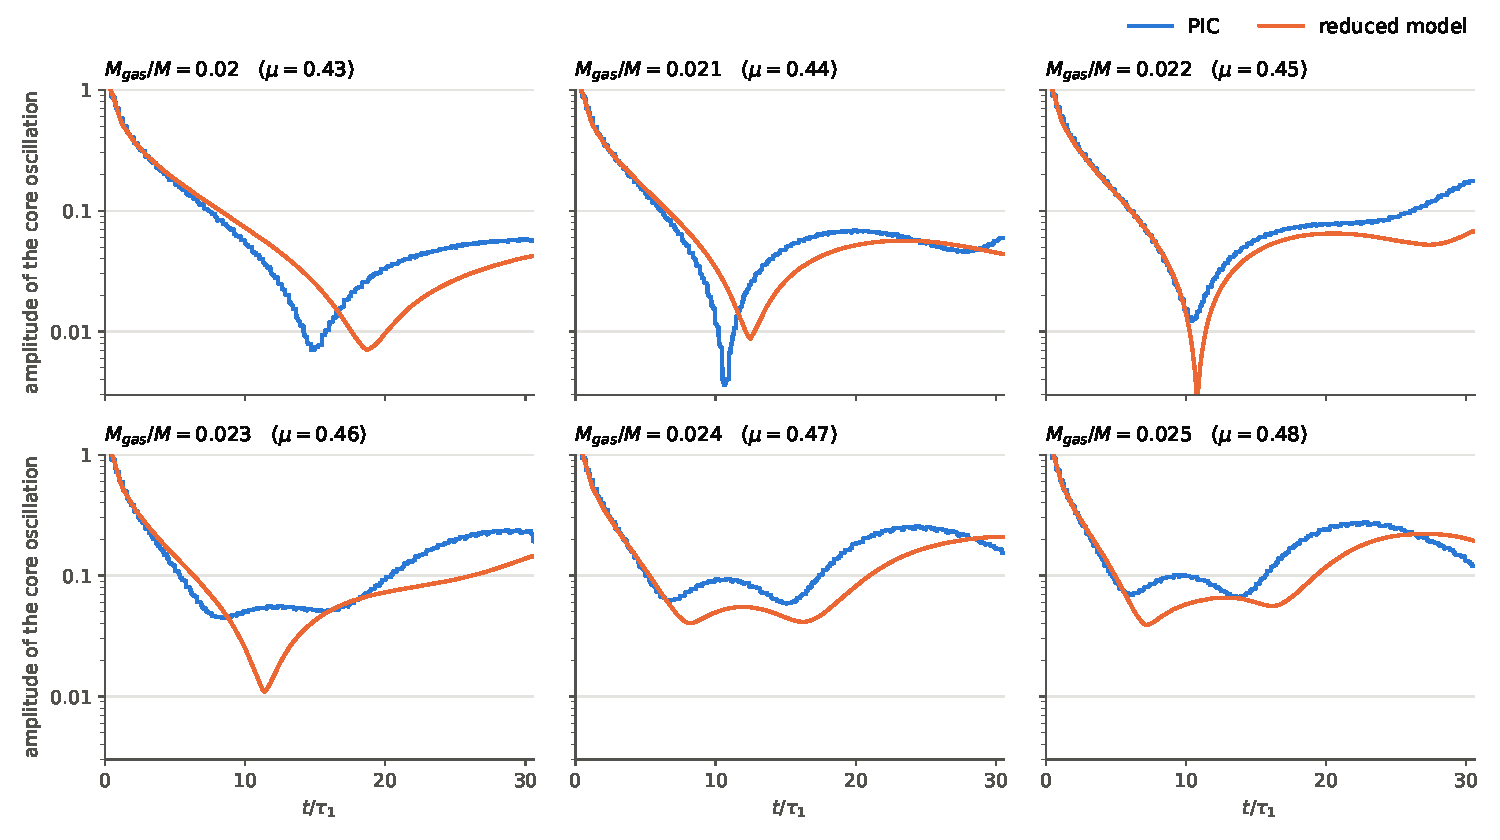
\includegraphics[width=\textwidth]{figuras/reducido_series.pdf}}
\caption{Amplitude of the radial oscillation of the core for the six masses of the reference family between $\mu = 0.43$ and $\mu = 0.48$: PIC simulations (envelope of the deviation of the mean radius of the core from its average over one radial period) and reduced model ($|\zeta_c|/\sqrt{\kappa_0}$).}
\label{Fig:Series}
\end{figure}

\begin{figure}[htp]
\centerline{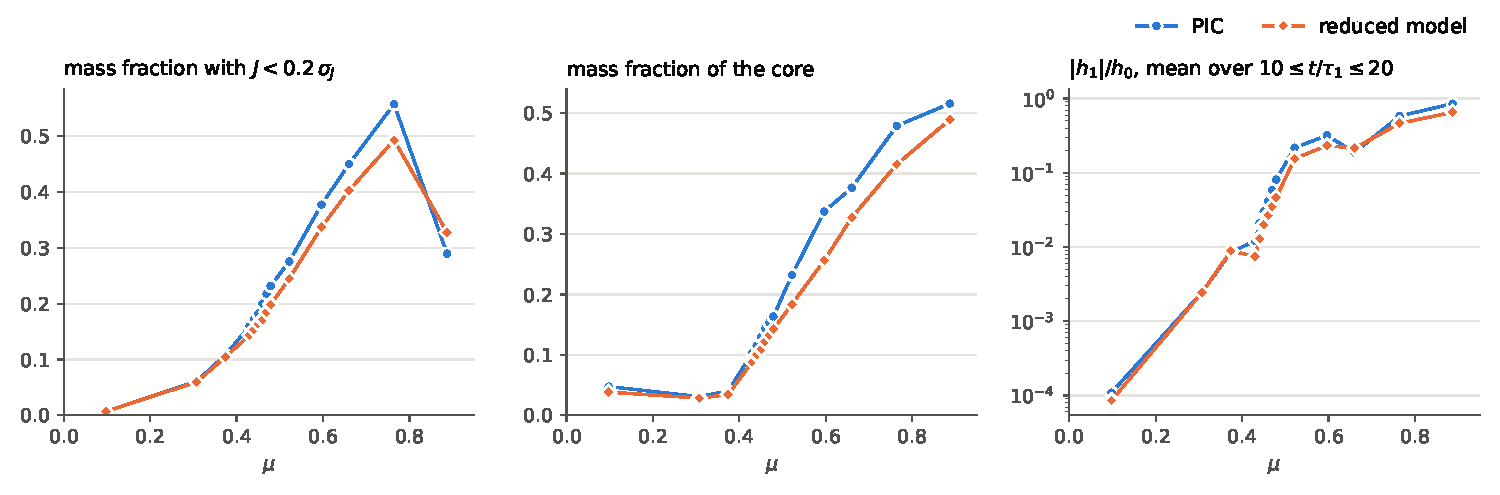
\includegraphics[width=\textwidth]{figuras/reducido_estado.pdf}}
\caption{State of the gas at late times for the reference family as a function of $\mu$: PIC simulations and reduced model. The quantities are those of Table~\ref{Tab:Reference}.}
\label{Fig:State}
\end{figure}

Table~\ref{Tab:Reference} and Figs.~\ref{Fig:Series} and~\ref{Fig:State} compare the solutions of Eq.~(\ref{Eq:Reduced}) with the PIC simulations of the reference family. The agreement depends on $\mu$ as follows.

For $\mu\leq 0.37$, where the gas mixes, the model reproduces $|h_1|$ and the mass which accumulates near the circular orbit within $2$ to $4$ percent; for $M_{gas}/M = 10^{-3}$ the value of $|h_1|$ is at the level of the numerical noise of both computations. In particular, the model reproduces the fact that the mixed state differs from the average of the initial DF over the angle variable: for $M_{gas}/M = 0.01$ the fraction of the mass with $J < 0.2\,\sigma_J$ is $0.060$, compared with $0.061$ in the PIC simulation and with $0.005$ in the absence of self-gravity. The distribution of the action variables near the circular orbit also agrees: in the six intervals of width $0.01\,\sigma_J$ between $J = 0$ and $J = 0.06\,\sigma_J$ the mass per unit of $J/\sigma_J$ is $0.025$, $0.070$, $0.119$, $0.164$, $0.222$ and $0.247$ in the model and $0.025$, $0.072$, $0.117$, $0.165$, $0.223$ and $0.247$ in the PIC simulation, in units of $M_{gas}$. Hence, the density of the mixed state grows linearly with $J$ near the circular orbit, whereas the initial one is proportional to $J^2$.

For $0.43\leq\mu\leq 0.48$ the model reproduces the formation of the core and the evolution of its oscillation: the first decay of the amplitude, its minimum and its subsequent growth, see Fig.~\ref{Fig:Series}. In both computations all the quantities change continuously with $\mu$ in this range, and $|h_1|$ grows by a factor between $1.3$ and $1.7$ for each increase of $M_{gas}/M$ by $10^{-3}$. The values of the model are those of the PIC simulations with a mass which is smaller by $4$ to $8$ percent: $|h_1|$ is $0.6$ times and $m_c$ is $0.87$ times the one of the PIC simulations with the same mass. The root mean square radial extension of the core is the same, between $0.14$ and $0.16$ in both. The frequency of the oscillation of the core in the model, relative to $\kappa_0$, is $9.1\times 10^{-4}$ for $2\leq t/\tau_1\leq 14$ and $7.9\times 10^{-4}$ for $22\leq t/\tau_1\leq 30$ for $M_{gas}/M = 0.02$; subtracting $\kappa_0$ and the uniform shift from the values of Table~\ref{Tab:Frequencies} gives $7.7\times 10^{-4}$ and $6.8\times 10^{-4}$ for the PIC simulation. The gap in the distribution of the action variables at the resonance is also present in the model, between $0.07\,\sigma_J$ and $0.12\,\sigma_J$, although it is less deep ($35$ to $40$ percent of the density of the halo).

For $\mu = 0.52$ the model reproduces the modulation of the amplitude of the core during the whole simulation (minimum $0.10$ at $t\approx 5\tau_1$ to $10\tau_1$, maximum $0.29$ at $t\approx 18\tau_1$, and a second minimum of $0.06$ at $t\approx 25\tau_1$, compared with $0.12$, $0.32$ and $0.09$ in the PIC simulation). For $\mu\geq 0.60$ it gives the mass of the core within $10$ to $25$ percent and the correct level of the oscillation, but not its details, and for $\mu = 0.89$, where the mass of the gas is one tenth of the central mass, the amplitude of the core decreases from $0.9$ to $0.65$ in the model while it remains at $1.05$ in the PIC simulation.


\subsection{Other widths and the Kepler potential}
\label{SubSec:CompFam}

\begin{table}[htp]
\begin{tabular}{|l|c|c||c|c||c|c||c|c|}\hline
 & & & \multicolumn{2}{c||}{$|h_1|/h_0$} & \multicolumn{2}{c||}{mass with $J < 0.2\,\sigma_J$} & \multicolumn{2}{c|}{$m_c$} \\
Family & $M_{gas}/M$ & $\mu$ & PIC & model & PIC & model & PIC & model \\\hline
\TabFamilias
\end{tabular}
\caption{Same as Table~\ref{Tab:Reference} for the cloud in the Kepler potential and for the clouds with other widths in the isochrone potential; the parameters which are not indicated are those of the reference family. The value of $m_c$ is given when both computations yield a compact core. In each case the reduced model uses the lattice of the PIC simulation.}
\label{Tab:Families}
\end{table}

Table~\ref{Tab:Families} shows the same comparison for the remaining $18$ PIC simulations of the main notes. In the regime in which the gas mixes ($\mu\leq 0.4$) the model reproduces $|h_1|$ within $10$ to $15$ percent, except for the two smallest values, and the mass near the circular orbit within $5$ to $10$ percent, in all the families.

The dependence on the width in the angle variable is reproduced. For $\mu = 0.52$ the cloud with $\sigma_Q = 0.4$ leaves a core with $8$ percent of the mass and $|h_1|\approx 10^{-2}$, whereas in the reference family the core contains $23$ percent of the mass and $|h_1| = 0.22$; the model gives $7$ and $18$ percent, respectively. For $\sigma_Q = 0.2$ and $\mu = 0.42$ the amplitude of the oscillation of the core in the model differs by less than $10$ percent from the one of the PIC simulation at the $14$ times between $\tau_1$ and $30\tau_1$ at which they were compared. Hence, the model accounts for the fact that a cloud which is wide in the angle variable requires a larger value of $\mu$, which is not captured by the parameter $\mu$ nor by the estimate~(\ref{Eq:muEstimate}).

In the Kepler potential the agreement is the same as in the isochrone potential. The dependence on $\sigma_J$ shows the limit of the model: the mass of the core differs from the one of the PIC simulations by $5$ percent for $\sigma_J = 0.05$, by $15$ to $20$ percent for $\sigma_J = 0.1$ and by $35$ percent for $\sigma_J = 0.2$. The ratio between the amplitude of the radial oscillation and $R_0$ is $0.21$, $0.29$ and $0.41$ in these three cases, such that the error grows with the eccentricity of the orbits, as expected from an expansion to leading order in this ratio. For $\sigma_J = 0.05$ the model remains accurate up to $\mu = 0.69$, where it gives $|h_1| = 0.26$ and $m_c = 0.334$, compared with $0.27$ and $0.353$.

\subsection{Long times}
\label{SubSec:CompLong}

\begin{table}[htp]
\begin{tabular}{|c|c|c||c|c|c|c|c|c|}\hline
 & & & \multicolumn{6}{c|}{mean value of $|h_1|/h_0$ over the interval of $t/\tau_1$} \\
$M_{gas}/M$ & $N_J\times N_Q$ & $N_{eff}$ & $[10,20]$ & $[20,30]$ & $[30,40]$ & $[40,60]$ & $[60,80]$ & $[80,100]$ \\\hline
\TabLargas
\end{tabular}
\caption{Solutions of the reduced model~(\ref{Eq:Reduced}) up to $t = 100\tau_1$ for the reference cloud. The effective number of particles is $N_{eff} := (\sum_j m_j)^2/\sum_j m_j^2$; a set of $N_{eff}$ particles with random angles gives $|h_1|/h_0\approx N_{eff}^{-1/2}$, which is $0.067$, $0.045$ and $0.033$ for the three lattices.}
\label{Tab:Long}
\end{table}

The PIC simulations extend over $30\tau_1$, and they do not show whether the oscillation of the core is eventually damped. Since the reduced model is cheaper, we have solved it up to $t = 100\tau_1$ for four masses of the reference family, and for two of them with three different lattices, see Table~\ref{Tab:Long}. In none of the cases does the oscillation disappear. For $\mu = 0.52$ the value of $|h_1|$ decreases slowly, from $0.16$ to $0.07$, and the mass of the core remains at $0.18$. For $\mu = 0.43$ it increases after the minimum of the amplitude: the three lattices agree up to $t = 40\tau_1$, and the two finer ones up to $t = 60\tau_1$, where $|h_1|$ has grown from $0.007$ to $0.036$. At later times the results depend on the lattice, and for all the masses they approach values between $0.045$ and $0.07$, which are between $1.4$ and $2.1$ times the value $N_{eff}^{-1/2} = 0.033$ that corresponds to particles with random angles. Hence, for $t > 60\tau_1$ the solutions are affected by the finite number of particles, and they do not allow us to decide whether the oscillation of the core persists indefinitely in the limit $N\to\infty$. Answering this question requires more particles than the direct sum over the pairs permits. \EJ{A faster evaluation of the sums (tree or grid) would allow $10^5$ particles. The comparison for distributed angular momenta of section~\ref{Sec:DistL} with the PIC code is also missing.}


%%%%%%%%%%%%%%%%%%%%%%%%%%%%%%%%%%%%%%%%%%%%%
\section{Conclusions}
\label{Sec:Conclusions}
%%%%%%%%%%%%%%%%%%%%%%%%%%%%%%%%%%%%%%%%%%%%%

In these notes we have derived a reduced model for a self-gravitating gas cloud whose particles move on nearly circular orbits in an external central potential, and we have compared it with the PIC simulations of the main notes.

For gas particles with the same angular momentum the model is given by Eq.~(\ref{Eq:Reduced}). It describes the transport of the mass density in the plane of the complex amplitudes of the radial oscillations by a flow which consists of the differential rotation due to the external potential and of the rotation which is induced by the gas itself. For a cloud of a given shape it contains the single parameter~(\ref{Eq:Gamma}), which is proportional to the square of the parameter $\mu$ of the main notes. The model explains why the core forms at the circular orbit, where the differential rotation vanishes, it gives the frequencies of the mixed states and of the oscillation of the core, and it locates the resonance between this oscillation and the gas particles of the halo, at which the PIC simulations show a gap in the distribution of the action variables. Without adjusting any parameter, its solutions reproduce the $48$ PIC simulations with the accuracy described in section~\ref{Sec:Comparison}: a few percent when the gas mixes, a displacement of $4$ to $8$ percent in the mass in the range of $\mu$ in which the oscillation of the core becomes persistent, and $10$ to $35$ percent in the mass of the core for the largest masses and the widest clouds in the action variable. Both computations agree in that the change between the relaxed state and the persistent oscillation is continuous in $\mu$.

The model has the following limitations. It is of leading order in the eccentricity of the orbits, and its error grows with the width of the cloud in the action variable. It does not provide the damping rate of the oscillation of the core nor the mass of the core in closed form; these are obtained from its numerical solution. Its solutions up to $100\tau_1$ do not show a decay of the oscillation of the core, but beyond $60\tau_1$ they are limited by the number of particles. For distributed angular momenta the model is given by Eq.~(\ref{Eq:ReducedL}), in which the interaction is softened by the spread of the circular orbits. Its solutions predict that for $\mu = 0.52$ the oscillation of the core is lost when the width of the distribution of the angular momenta reaches $0.7$ percent of $L_0$ and that no core is left at $1.4$ percent, which would restrict the results of the main notes on the core to gas clouds with almost equal angular momenta. This prediction has not been compared with simulations yet, and it is the most important point to be settled. Finally, the interaction of the reduced model is the one of the self-gravitating sheet model, which also describes the motion perpendicular to a galactic disk; whether Eq.~(\ref{Eq:Reduced}) is useful in that context, where the potential in which the stars oscillate is generated by the disk itself, remains to be analyzed.


\bibliographystyle{unsrt}
\bibliography{refs}

\end{document}
